%%%%%%%%%%%%%%%%%%%%%%%%%%%%%%%%%%%%%%%%%%%%%%%%
% Template productivity report
% 
% Alberto Sanchez asanchezrodelgo@ifc.org May 2016
%%%%%%%%%%%%%%%%%%%%%%%%%%%%%%%%%%%%%%%%%%%%%%%%
\documentclass{article}\usepackage[]{graphicx}\usepackage[]{color}
%% maxwidth is the original width if it is less than linewidth
%% otherwise use linewidth (to make sure the graphics do not exceed the margin)
\makeatletter
\def\maxwidth{ %
  \ifdim\Gin@nat@width>\linewidth
    \linewidth
  \else
    \Gin@nat@width
  \fi
}
\makeatother

\definecolor{fgcolor}{rgb}{0.345, 0.345, 0.345}
\newcommand{\hlnum}[1]{\textcolor[rgb]{0.686,0.059,0.569}{#1}}%
\newcommand{\hlstr}[1]{\textcolor[rgb]{0.192,0.494,0.8}{#1}}%
\newcommand{\hlcom}[1]{\textcolor[rgb]{0.678,0.584,0.686}{\textit{#1}}}%
\newcommand{\hlopt}[1]{\textcolor[rgb]{0,0,0}{#1}}%
\newcommand{\hlstd}[1]{\textcolor[rgb]{0.345,0.345,0.345}{#1}}%
\newcommand{\hlkwa}[1]{\textcolor[rgb]{0.161,0.373,0.58}{\textbf{#1}}}%
\newcommand{\hlkwb}[1]{\textcolor[rgb]{0.69,0.353,0.396}{#1}}%
\newcommand{\hlkwc}[1]{\textcolor[rgb]{0.333,0.667,0.333}{#1}}%
\newcommand{\hlkwd}[1]{\textcolor[rgb]{0.737,0.353,0.396}{\textbf{#1}}}%

\usepackage{framed}
\makeatletter
\newenvironment{kframe}{%
 \def\at@end@of@kframe{}%
 \ifinner\ifhmode%
  \def\at@end@of@kframe{\end{minipage}}%
  \begin{minipage}{\columnwidth}%
 \fi\fi%
 \def\FrameCommand##1{\hskip\@totalleftmargin \hskip-\fboxsep
 \colorbox{shadecolor}{##1}\hskip-\fboxsep
     % There is no \\@totalrightmargin, so:
     \hskip-\linewidth \hskip-\@totalleftmargin \hskip\columnwidth}%
 \MakeFramed {\advance\hsize-\width
   \@totalleftmargin\z@ \linewidth\hsize
   \@setminipage}}%
 {\par\unskip\endMakeFramed%
 \at@end@of@kframe}
\makeatother

\definecolor{shadecolor}{rgb}{.97, .97, .97}
\definecolor{messagecolor}{rgb}{0, 0, 0}
\definecolor{warningcolor}{rgb}{1, 0, 1}
\definecolor{errorcolor}{rgb}{1, 0, 0}
\newenvironment{knitrout}{}{} % an empty environment to be redefined in TeX

\usepackage{alltt}
%%%%%%%%%%%%%% package declaration %%%%%%%%%%%%%%%%%%%%%
\usepackage{fancyhdr}
\pagestyle{fancy}
\lhead{This is my name}
\rhead{this is page \thepage}
\cfoot{center of the footer!}
\usepackage[top=0.3in, bottom=0.1in, left=0.5in, right=0.6in]{geometry}
\usepackage{graphicx} % to load images
\usepackage[export]{adjustbox} % add alignment to includegraphics
\usepackage[font=small]{caption}
\usepackage{xcolor} % color text
\usepackage{tabularx} % to adjust table width, etc. 
\usepackage{titlesec} % format titles and headers
\usepackage{sectsty} % format sections & subsections
\usepackage{booktabs} % For \toprule, \midrule and \bottomrule
\usepackage{longtable} % add pages for long tables
\usepackage[colorlinks = true,
            linkcolor = blue,
            urlcolor  = blue,
            citecolor = blue,
            anchorcolor = blue]{hyperref} % to include hyperlinks in the doc
\sectionfont{\fontsize{24}{22}\selectfont\raggedright} % formats title newsletter (section) 
\subsectionfont{\fontsize{14}{12}\selectfont\raggedright} % formats title newsletter (section)
%%%%%%%%%%%%%%%%%%%%%%%%%%%%%%%%%%%%%%%%%%%%%%%%%%%%%%%%%%%%%%%%%%%%%%%%%%%%%%%%%%%
%
%%%%%%%%%%%%%%%%%%%%%%%%%%%%%%%%%%%%% BEGIN DOCUMENT %%%%%%%%%%%%%%%%%%%%%%%%%%%%%%
\IfFileExists{upquote.sty}{\usepackage{upquote}}{}
\begin{document}

%

%%%%%%%%%%%%%%%% PAGE 1 %%%%%%%%%%%%%%%%%%%
%World Bank logo and TCMN branding
\begin{figure}
  \vspace{-3ex} % move up this figure
  \hspace{-7ex} % move left this figure
  \includegraphics[width=5cm]{/Users/asanchez3/shinyTCMN/www/wb_logo_background.png}
\end{figure}
%\begin{figure}
 \begin{minipage}[t]{1.1\textwidth} % top section
      \vspace{-30ex}
      \hspace{10ex}
      \raggedleft{\section*{\color{white!20!black}Productivity Indicators Report}}
      %\raggedright{\includegraphics[width=5.5cm,right]{/Users/asanchez3/shinyTCMN/www/TC_snapshots_operations.png}}
  \end{minipage}
  
%\end{figure}
%
%%%% Macro Indicators
\begin{minipage}[t]{0.99\textwidth} % top section
  \vspace{-0.5cm}
      \subsection*{\color{white!40!black}Sector: \color{blue!40!black}All sectors}
      \subsection*{\color{white!40!black}Firm type: \color{blue!40!black}All firms}
      \subsection*{\color{white!40!black}Indicator: \color{blue!40!black}sales (d2) over labor (l1) (in 2009 USD)}
  \end{minipage} % end top section

\vspace*{1.5cm}
  \raggedright{\color{white!30!black} \textbf{\Large Summary Statistics}}
    \begin{minipage}[c]{0.99\textwidth}  
      \vspace*{0.2cm}
      
% latex table generated in R 3.2.2 by xtable 1.7-4 package
% Sun May  1 16:16:08 2016
\begin{tabular}{lrrrl}
  & median\_sum & sd\_sum & iqr\_sum &  \\ 
  \hline
Min & 744.43 & 3223.80 & 2200.55 &  \\ 
  Max & 6324166.71 & 25030364.04 & 38726905.76 &  \\ 
  Mean & 91886.25 & 376434.76 & 494759.66 &  \\ 
  Median & 21524.77 & 32745.85 & 31128.90 &  \\ 
  Stdev & 607753.03 & 2584244.82 & 3821305.17 &  \\ 
  IQR & 31186.71 & 40638.61 & 40329.88 &  \\ 
  \end{tabular}

      \vspace*{0.5cm}
    \end{minipage}
    
    \begin{minipage}[c]{0.99\textwidth}  


{\centering 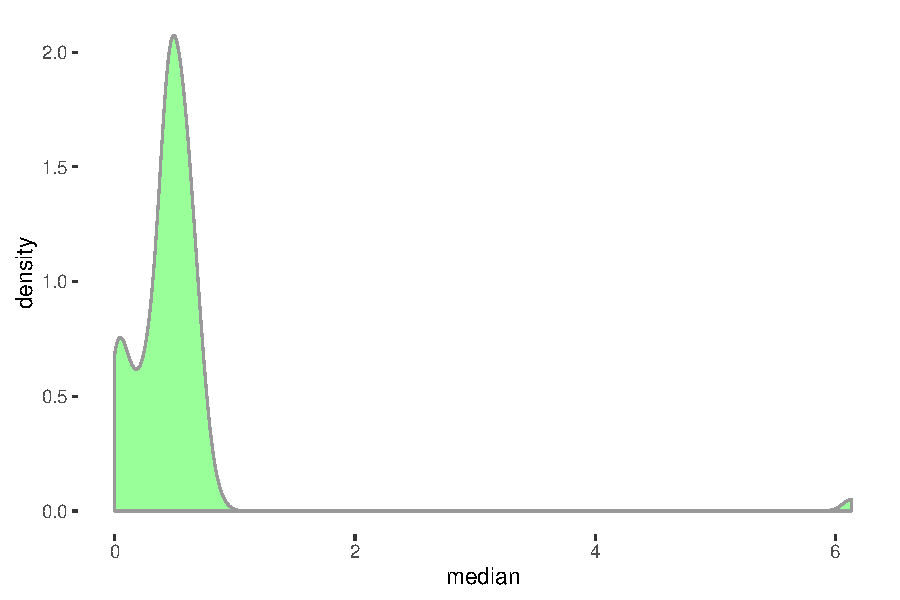
\includegraphics[width=\maxwidth]{figure/plot2-1} 

}



      \vspace*{0.5cm}
    \end{minipage}
%\end{minipage}

\newpage

  \raggedright{\color{white!30!black} \textbf{\Large Income Level Statistics}}
    \begin{minipage}[c]{0.99\textwidth}  
      \vspace*{0.4cm}
      
% latex table generated in R 3.2.2 by xtable 1.7-4 package
% Sun May  1 16:16:12 2016
\begin{tabular}{lrrrl}
  & median & sd & iqr &  \\ 
  \hline
Low income & 4981.38 & 10085.95 & 8689.39 &  \\ 
  Lower middle income & 12368.33 & 18718.40 & 18846.25 &  \\ 
  Upper middle income & 29072.07 & 44111.15 & 45370.12 &  \\ 
  High income & 50000.00 & 76406.04 & 85549.60 &  \\ 
  \end{tabular}

      \vspace*{1cm}
    \end{minipage}
    
    \begin{minipage}[c]{0.99\textwidth}  
    


{\centering 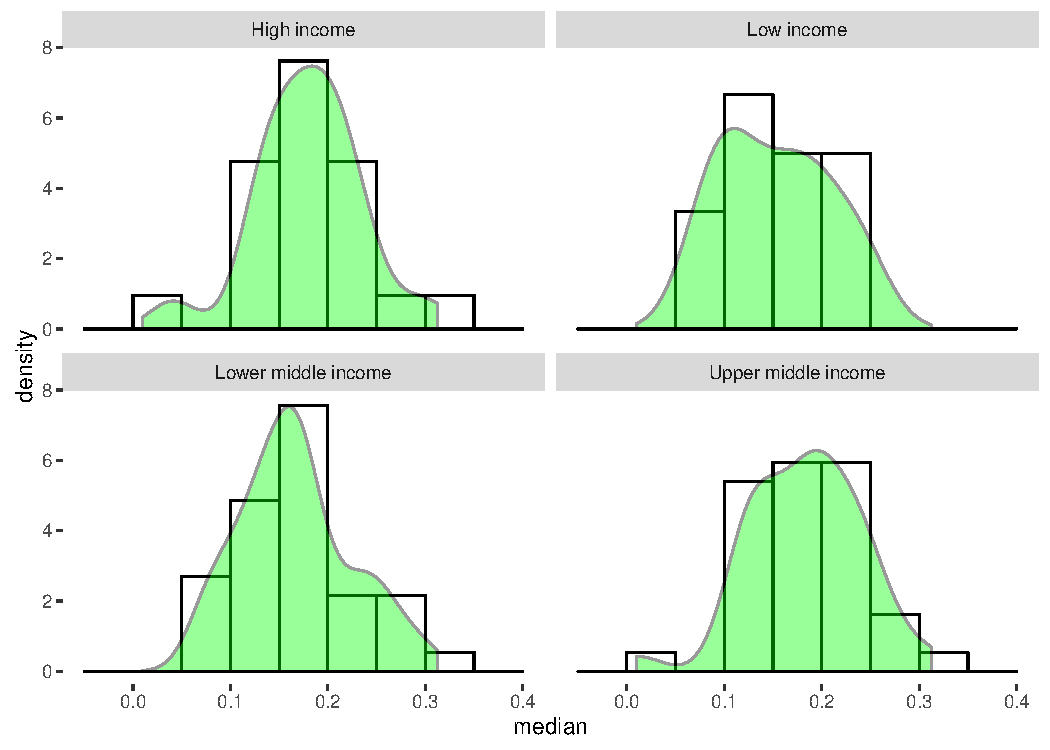
\includegraphics[width=\maxwidth]{figure/plot3-1} 

}



      \vspace*{0.5cm}
    \end{minipage}
%\end{minipage}

\newpage

  \raggedright{\color{white!30!black} \textbf{\Large Region Level Statistics}}
    \begin{minipage}[c]{0.99\textwidth}  
      \vspace*{0.4cm}
      
% latex table generated in R 3.2.2 by xtable 1.7-4 package
% Sun May  1 16:16:34 2016
\begin{tabular}{lrrrl}
  & median & sd & iqr &  \\ 
  \hline
East Asia and Pacific & 14098.92 & 20633.05 & 23947.90 &  \\ 
  Europe and Central Asia & 32468.93 & 46800.19 & 50345.23 &  \\ 
  Latin America and Caribbean & 31128.69 & 33876.29 & 37131.89 &  \\ 
  Middle East and North Africa & 27548.57 & 58865.32 & 53120.11 &  \\ 
  South Asia & 5135.13 & 12814.63 & 9248.39 &  \\ 
  Sub-Saharan Africa & 7412.38 & 19090.88 & 19899.36 &  \\ 
  \end{tabular}

      \vspace*{1cm}
    \end{minipage}
    
    \begin{minipage}[c]{0.99\textwidth}  
    


{\centering 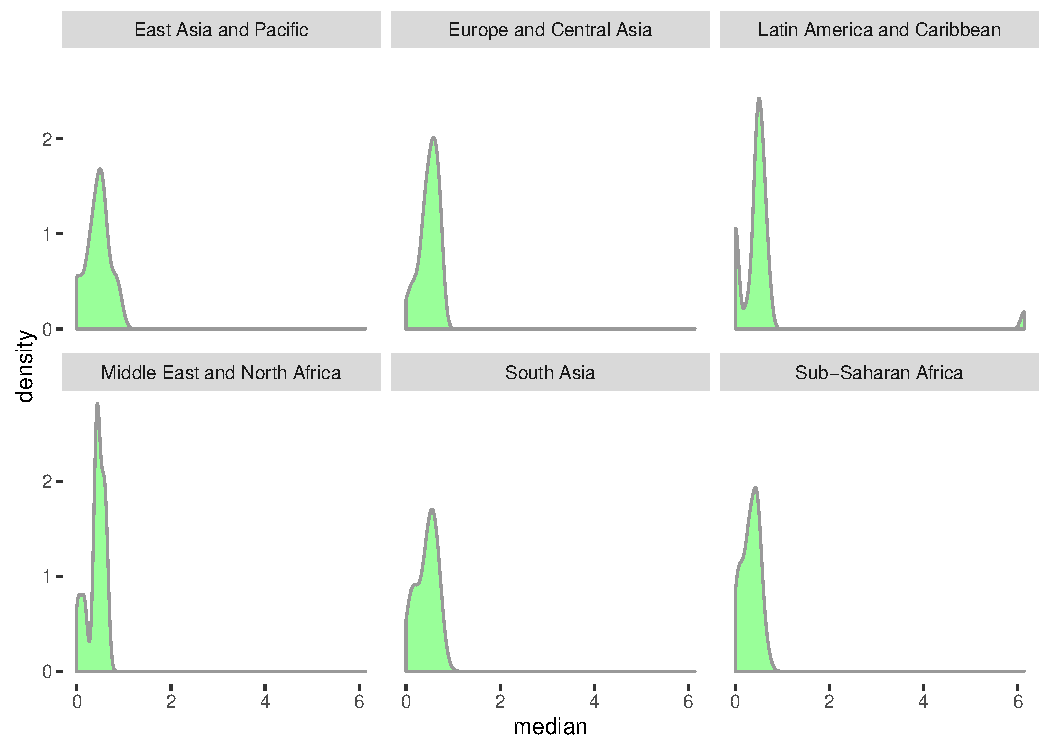
\includegraphics[width=\maxwidth]{figure/plot4-1} 

}



      \vspace*{0.5cm}
    \end{minipage}
%\end{minipage}

%%%%%%%%%%%%%%%% END OF DOCUMENT %%%%%%%%%%%%%%%%%%%
\end{document}
